\documentclass[sigconf]{acmart}

\usepackage{graphicx}
\usepackage{hyperref}
\usepackage{todonotes}

\usepackage{endfloat}
\renewcommand{\efloatseparator}{\mbox{}} % no new page between figures

\usepackage{booktabs} % For formal tables

\settopmatter{printacmref=false} % Removes citation information below abstract
\renewcommand\footnotetextcopyrightpermission[1]{} % removes footnote with conference information in first column
\pagestyle{plain} % removes running headers

\newcommand{\TODO}[1]{\todo[inline]{#1}}

\begin{document}
\title{Big Data Analytics on Food Products Around the World}

\author{Karthik Vegi}
\affiliation{%
  \institution{Indiana University Bloomington}
  \streetaddress{College Mall Apartments}
  \city{Bloomington} 
  \state{Indiana} 
  \postcode{47401}
  }
\email{kvegi@iu.com}

\author{Nisha Chandwani}
\orcid{1234-5678-9012}
\affiliation{%
  \institution{Indiana University Bloomington}
  \streetaddress{Park Doral Apartments}
  \city{Bloomington} 
  \state{Indiana} 
  \postcode{47408}
}
\email{nchandwa@iu.edu}

% The default list of authors is too long for headers}
\renewcommand{\shortauthors}{kvegi, nchandwa}

\begin{abstract}
Food is one of the basic necessities of human-being. It helps us gain energy to recharge our body to do the daily activities like moving, playing, and thinking. From being a cave man to producing wide variety of foods, we have come a long way. The civilizations shaped the food habits of the world and there is a lot of variance in the food habits across countries. We analyze the {\em Open Food Facts} database that gathers information on food products from around the world to unearth some food habits of the world and we predict the food grade based on the nutrition facts of the food products.
\end{abstract}

\keywords{i523, hid231, hid203, big data, food habits, food products, nutrition}

\maketitle

\section{Introduction}
{\em Open Food Facts} is a non-profit initiative started by Stephane Gigandet and run by thousands of volunteers around the world. Any person around the world can contribute to the database by simply scanning a product using a mobile app which is made available to IOS and Android. This massive database of food products opens up a lot of opportunities to analyze the food products around the world and understand their food habits. We are particularly interested in the consumption of nutrients that come along with the food items across the world, the composition of different fat content, and the prediction of nutrition grade based on the nutrients.

\section{Food Analysis: Importance and Related work}
In recent times, more and more companies try to market their food as low-fat or low-calories in order to fool consumers into buying their products. The increasing concern of public health has led to a significant interest in detecting the health-related properties of food products  \cite{cifuentes2012food}. Thus, there is no question about the importance of analysis of the nutrition grade and food safety in today's world. The analysis of food requires more robust and efficient methodologies in order to ensure the quality and safety of the food products \cite{cifuentes2012food}. Previous methods based on the so-called wet-chemistry have now evolved into more powerful techniques which are used in the food laboratories These methods provide massive improvement in analytical accuracy thus expanding the limits of food applications \cite{cifuentes2012food}. The traditional methods of food analysis can be classified based on the underlying principle. Some of these categories are spectroscopic, biological, electrochemical, supercritical fluid chromatography \cite{cifuentes2012food}. All these techniques provide information about the sample under study and this information is derived from a specific physical-chemical interaction \cite{cifuentes2012food}. A different approach of analyzing and detecting the food quality is by using machine learning techniques. We will discuss one of these modern methods of food analysis which can be widely used across countries.


\section{Analysis of Fat content in Food}
Fat is definitely a nutrient that the body needs and are essential to aid in cell growth, help with energy generation, maintaining body temperature, protect organs, help absorb other essential nutrients that aid in producing energy, improve blood cholesterol level, help reduce inflammation in case of injury, and help in storing energy that can be used for survival when you go without food for few days \cite{www-health}. But, we do need to keep a track of the consumption because anything that is remotely excess leads to a variety of serious health issues \cite{www-health}.  

\subsection{Dietary Fats}
There are different types of fat – some are good and some are bad and some needs to be taken within a certain limit \cite{www-health}. 

\subsubsection{Saturated Fat}
More intake of saturated fats results in the cholesterol levels in the blood which increases the risk of heart related diseases \cite{www-health}. The American Heart Association suggests around 5 percent of daily calories from foods containing saturated fat \cite{www-health}. Meat, cheese and milk are some of the sources of saturated fat \cite{www-health}. 

\subsubsection{Trans Fat}
Any type of trans fat whether it is natural or artificial is not good \cite{www-health}. The reason why food manufacturers use trans-fat is because they are less expensive, can be produced artificially, easy to use with other ingredients, last for a long time and also aid in improving the taste of the food \cite{www-health}. Trans fats raise the bad fat levels and decreases the good fat levels \cite{www-health}. The American Heart suggests to completely cut off trans-fat from the diet \cite{www-health}.

\subsubsection{Monounsaturated Fat}
Monounsaturated fats have a good effect on the body when taken within limit \cite{www-health}. They help reduce the bad cholesterol levels in the blood and there by decrease the risk of heart diseases \cite{www-health}. They also help in gaining vitamin E which is a good nutrient that acts as antioxidant \cite{www-health}. Olive oil, avocados, and sesame oil are some of the sources for monounsaturated fats \cite{www-health}.

\subsubsection{Polyunsaturated Fat}
Polyunsaturated fats have a good effect on the body when taken within limit \cite{www-health}. They help reduce the bad cholesterol levels in the blood and there by decrease the risk of heart diseases \cite{www-health}. They also provide some nutrients that are essential for the body \cite{www-health}. Soybean oil and sunflower oil are some of the sources for polyunsaturated fats \cite{www-health}.

\subsection{Data Cleaning and Transformation}
To make the analysis more interesting, the top 20 countries with most value counts for the attributes have been considered. The countries with names combined with other countries were also cleaned in the process. The data set was analyzed was missing values and the attributes with more than 60 percent missing values were removed from the analysis to add consistency. Only the columns that are meaningful in the analysis were retained and the rest were removed from further analysis. \\

We then display the top 5 countries as a pie-chart and the 5 countries are namely United States, France, Switzerland, Germany, and Spain as shown in Figure \ref{fig:Fig7}. 

\begin{figure}
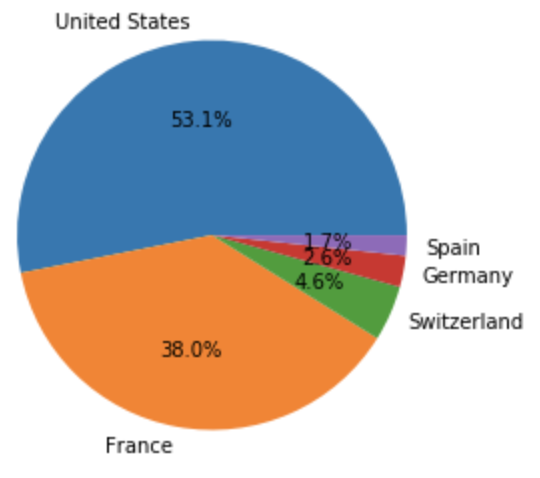
\includegraphics[width=1.0\textwidth]{images/fig7.png}
\caption{Top 5 countries \cite{code-base}}
\label{fig:Fig7}
\end{figure}

We then impute all the null values with zeroes and we then check the dietary fat content in the foods and check the top countries with fat content using a histogram. The analysis with respect to the fat countries is as follows \\

\subsection{Data Analysis}
The top 5 countries with most fat content in the food items are Serbia, United States, Switzerland, Germany, and Sweden as shown in Figure \ref{fig:Fig8}.
	
\begin{figure}
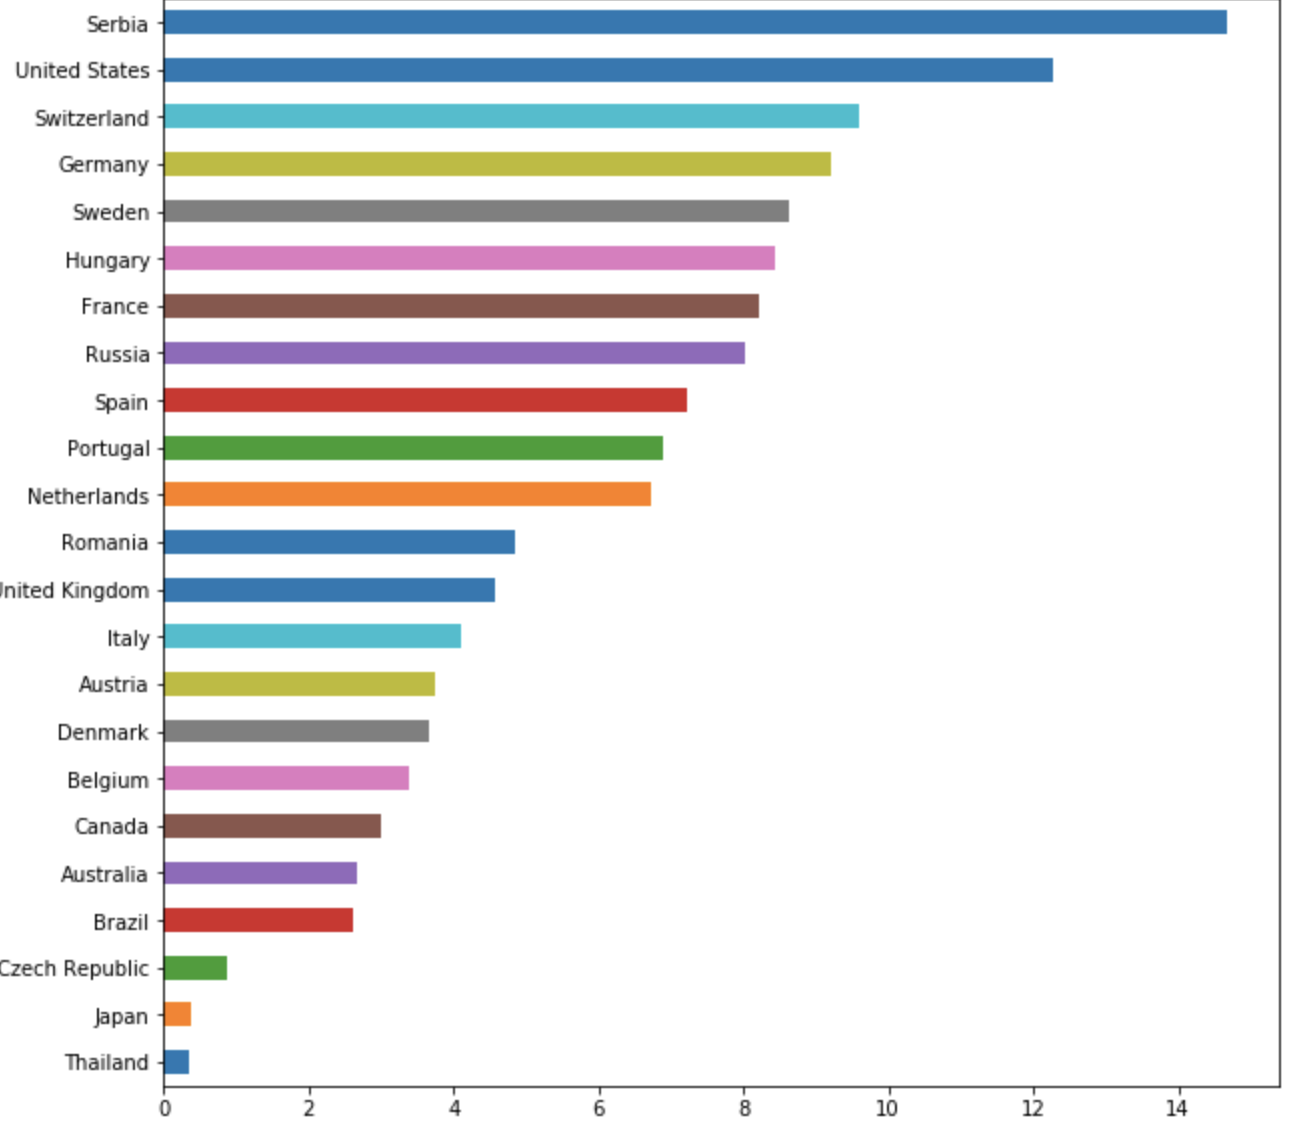
\includegraphics[width=1.0\textwidth]{images/fig8.png}
\caption{Top 5 countries with most fat content \cite{code-base}}
\label{fig:Fig8}
\end{figure}

The top 5 countries with most saturated fat content in the food items are Serbia, United States, Germany, France and Switzerland as shown in Figure \ref{fig:Fig9}
	
\begin{figure}
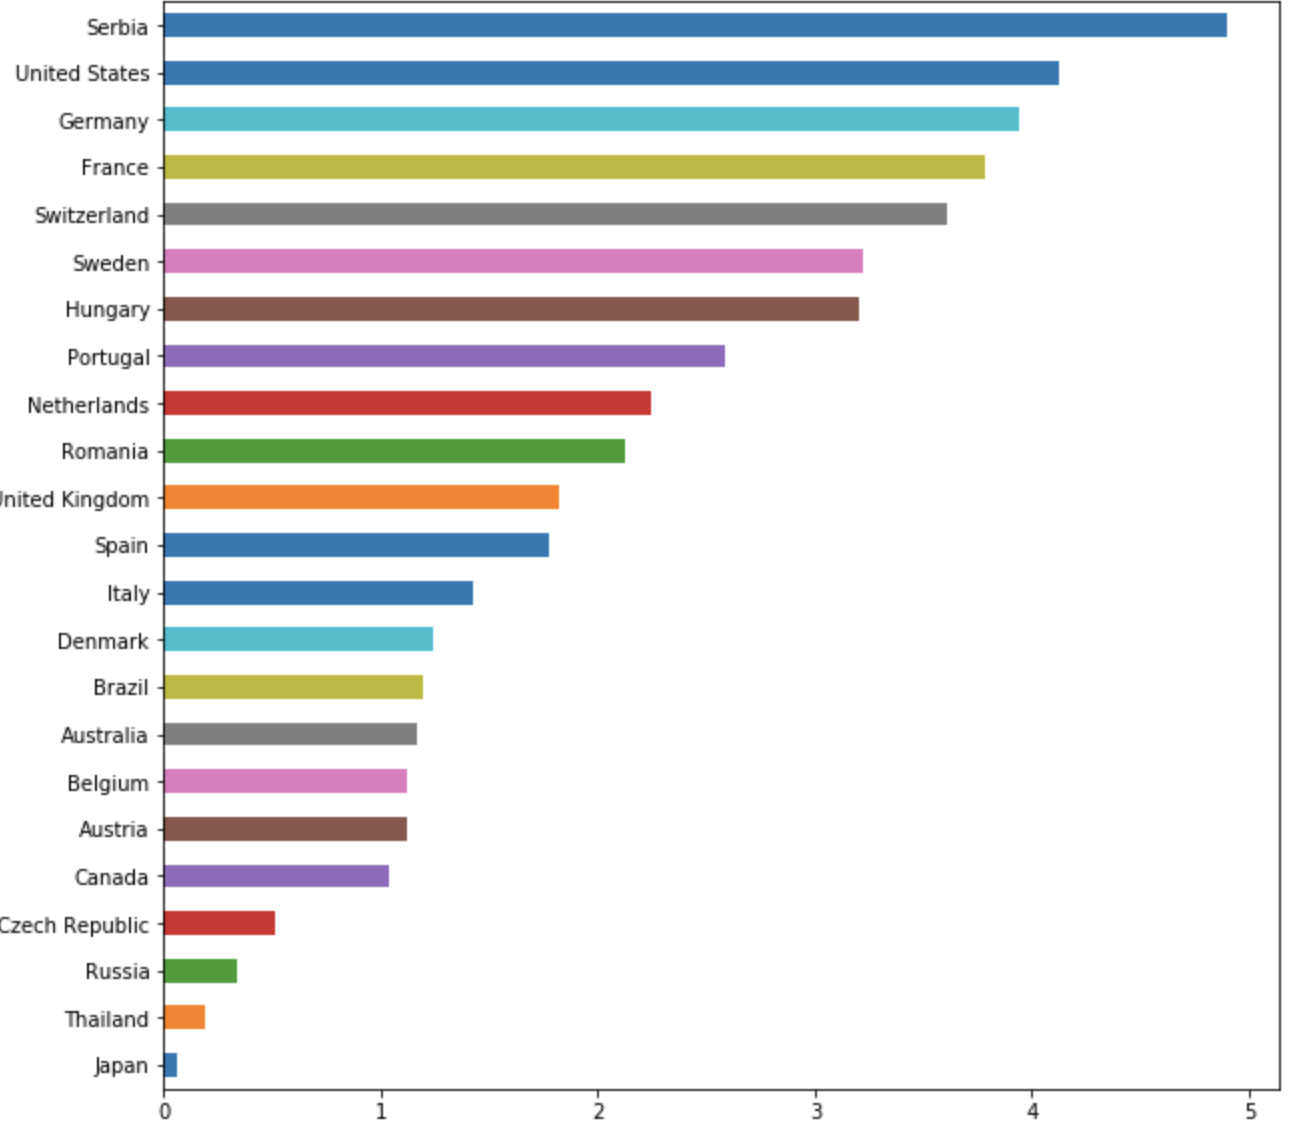
\includegraphics[width=1.0\textwidth]{images/fig9.png}
\caption{Top 5 countries with most saturated fat content \cite{code-base}}
\label{fig:Fig9}
\end{figure}

    
The top 5 countries with most trans-fat content in the food items are United States, Brazil, Canada, Australia, Russia, and Serbia as shown in Figure \ref{fig:Fig10} \\
	
\begin{figure}
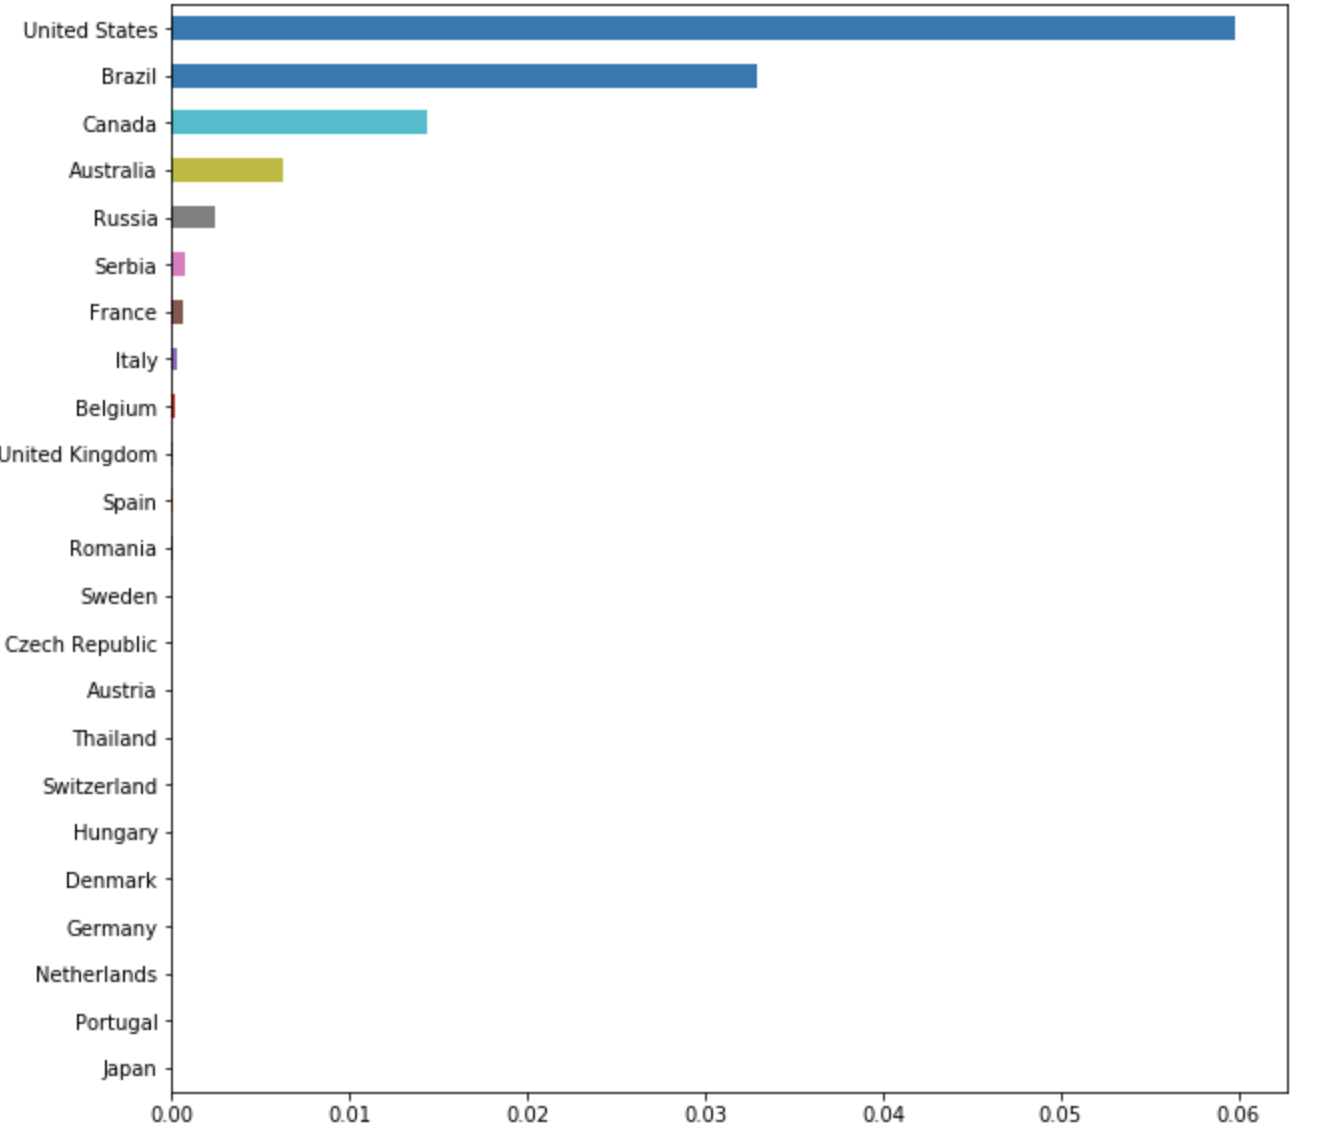
\includegraphics[width=1.0\textwidth]{images/fig10.png}
\caption{Top 5 countries with most trans-fat content \cite{code-base}}
\label{fig:Fig10}
\end{figure}
        
The top 5 countries with most cholesterol content in the food items are United States, Canada, Portugal, Brazil, France, and Italy as shown in Figure \ref{fig:Fig11} \\
	
\begin{figure}
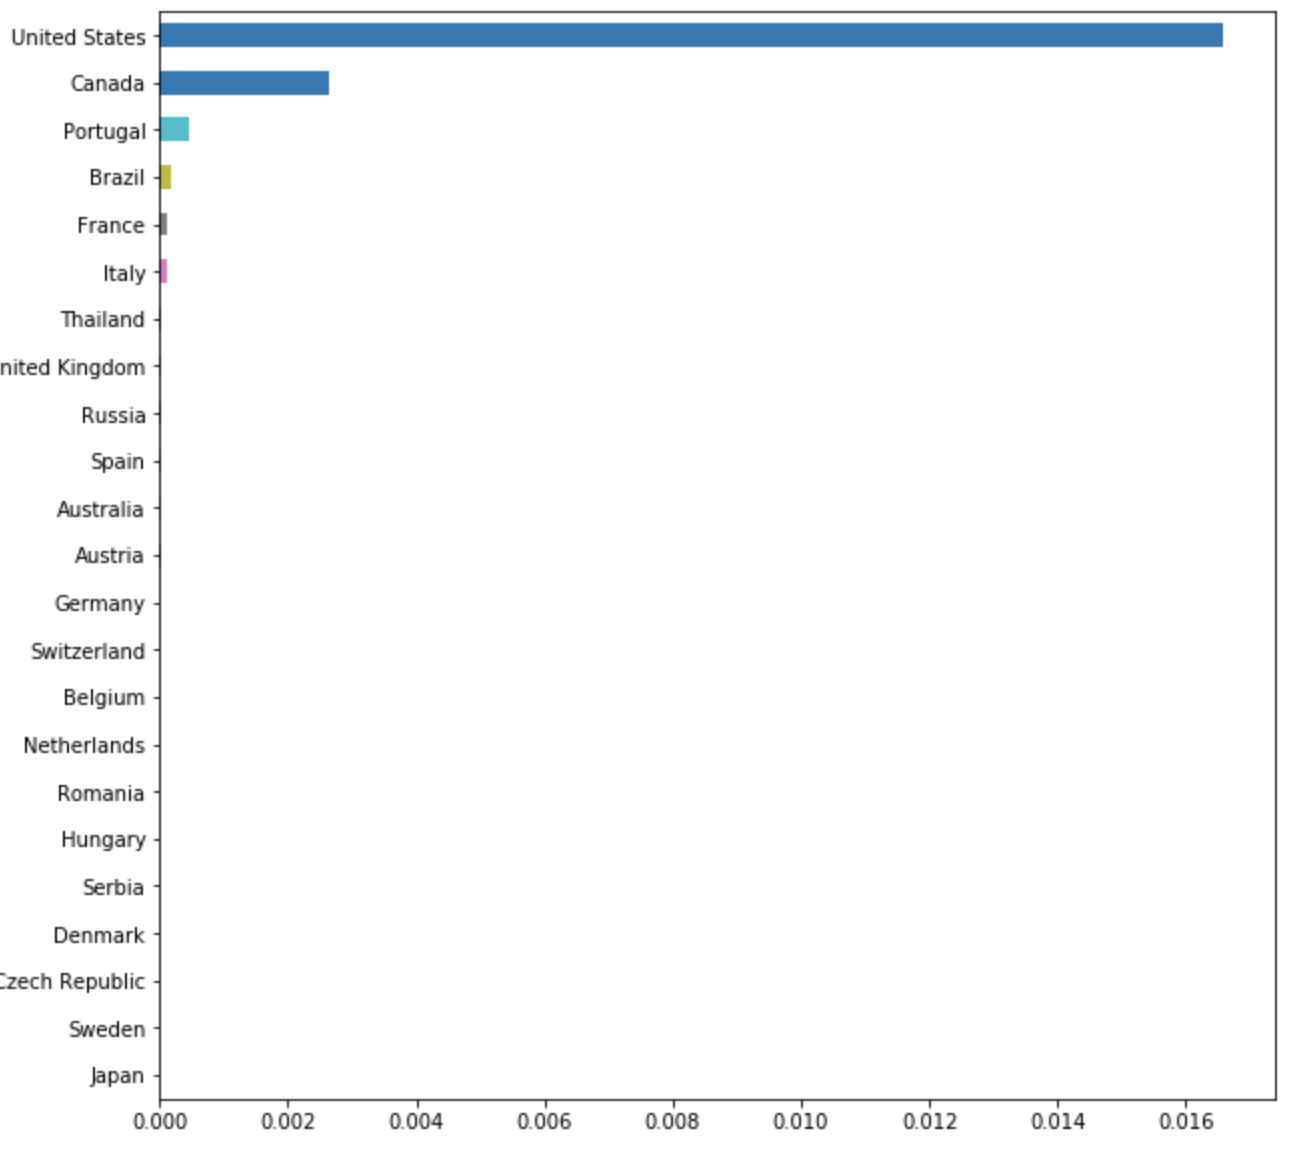
\includegraphics[width=1.0\textwidth]{images/fig11.png}
\caption{Top 5 countries with most cholesterol content \cite{code-base}}
\label{fig:Fig11}
\end{figure}

\section{Analysis of Sugar and Salt Content}

\section{Nutrition Grade Labelling System}
France recently took a decision to implement a nutri-score system which will use a color coding mechanism to label the food products that will help consumers know the nutrition grade of the product \cite{www-who}. The World Health Organization regional office for Europe as a part of its 5 year action plan from 2015-2020 recommends a labelling mechanism for the consumers to know about the quality of the food products at a first glance \cite{www-who}. This will not only make it easier for the consumers to pick healthier options but it will also regulate food manufacturers to resort to healthier ingredients instead of going for low cost artificial or less healthier ingredients \cite{www-who}.  \\

France after United Kingdom became the second country to implement this system to indicate the main ingredients like fat, salt and sugar content in the food items \cite{www-who}. France made use of an evidence based system to study different labelling systems to arrive at the best one \cite{www-who}. By implementing this system, the World Health Organization will keep a check on the growing number of diet related diseases in the Europe region \cite{www-who}. Europe being the largest consumer of cheese wants to regulate the ingredients that go into the manufacturing process so that people are well informed about their food choices \cite{www-who}.

\subsection{Nutrition Grade Prediction as a Big Data Problem}
We build a predictive classification model to predict the food nutrition grade based on the ingredients of the food. The goal is to apply various machine learning algorithms to the problem at hand, measure the prediction accuracy to compare and contrast the different algorithms, and arrive at the best algorithm that suits the given data and the problem. This problem can be solved using Big Data and Machine Learning techniques given the size and the complexity of the data.

\section{Machine Learning}
Machine Learning is a field in which we train computers in a way that they can learn from the input data \cite{book-shai}. The ideology is that computers use the training data that is made available to them, learn from it, build a model and use this experience to build knowledge that can be applied on new unseen data \cite{book-shai}. A wonderful example to demonstrate machine learning is the application to detect spam emails where the machine builds knowledge from previously seen emails which are marked as spam, checks new emails to see if they match the historic spam emails and label them as spam or non-spam \cite{book-shai}. 

\subsection{Types of Machine Learning Algorithms}
There are primarily two types of machine learning algorithms which are descriptive models and predictive models \cite{book-shai}. A {\em Descriptive Model} is described as the analysis done and insights gained from slicing and dicing the data in new and interesting ways \cite{book-shai}. One example of descriptive model is patter discovery that is often used in market basket analysis where transnational purchase details are analyzed \cite{book-shai}. A {\em Predictive Model} on the other hand involves predicting one value using one or more variables \cite{book-shai}. The learning algorithms tried to build a model that captures the relationship between a response variables and dependent target variables \cite{book-tan}.

\subsection{Types of Learning}
{\em Unsupervised Learning} is the process where there is no explicit training data to learn from, so there is simply no mechanism where the machine can learn from previously available data \cite{book-shai}. The same email example can be looked at in a different way where we now want to do anomaly detection in emails \cite{book-shai}. Here the main goal is to detect unusual messages from the bunch of messages and we do not have experience of previous data \cite{book-shai}. \\

{\em Supervised Learning} in contrast is the process of gaining knowledge or expertise from the training data which can be applied to future unseen data \cite{book-shai}. Here the model is first trained by using a bulk of training examples and this model is applied against testing data to measure the accuracy \cite{book-shai}. The variable that we need to predict is identified which is called the response variable and the variables that are used to predict the response variables, called the predictor variables are identified \cite{book-shai}. If the existing variables are not sufficiently giving the accuracy that is expected, a method called feature engineering is done where new variables are derived by combining existing variables \cite{book-shai}. 

\section{Prediction Analysis}
Prediction analysis is the process of working on  a large data set using a combination of statistical, data mining and machine learning algorithms to predict the outcome based on past data \cite{book-shai}.
There are primarily two types of prediction analysis in machine learning, namely regression and classification \cite{book-tan}. In regression, we try to predict a continuous variable from the predictor variables \cite{book-tan}. A good example of regression is to predict the housing prices from different parameters like year of construction, location, amenities, number of bed rooms etc \cite{book-tan}. Here the response variable is continuous and it is not predefined \cite{book-tan}. Classification on the other hand tries to predict a categorical variable in which we assign each record with a predefined label or a class \cite{book-tan}. \\

Classification is the task of assigning each data record to a predefined class \cite{book-tan}. In machine learning, classification is categorized as a supervised learning technique \cite{book-tan}. This problem has applications in various fields like spam detection, medical applications, astronomy and banking to identify fraudulent transactions from genuine transactions \cite{book-tan}. It is the task as coming up with a model which is essentially a function that maps every data record to a class label \cite{book-tan}. \\ 

The task at hand is a classification problem since we are trying to predict the food nutrition grade of the products based on the ingredients that go into the product. For this problem we are considering only the data for the country France, since the nutrition grade is available for most food products from the country. Another reason is that France is the first countries in the region to come up with the idea of adding a color coded label to the food products mentioning the nutrition grade. In the subsequent sections we discuss the machine learning techniques used to solve this problem.

\subsection{K Nearest Neighbors}

\subsubsection{Overview} Some of the classification algorithms in machine learning work on the principle of eager learning that involves a two step process where first a model is built from the training data and the model is applied on testing data \cite{book-tan}. In contrast, K nearest neighbors is a lazy learning algorithm where the process of modeling the training data is not done until the test examples are classified \cite{book-tan}. {\em Rote Classifier} is a good example of lazy learning algorithm memorizes the entire training data to perform classification but has the drawback of not being able to map every test example against the training example \cite{book-tan}. K nearest neighbors algorithm overcomes this drawback by finding all the records that are closest or nearest to the training records \cite{book-tan}. \\

The nearest neighbour puts each attribute list as a data point in the n-dimensional space, given n the number of attributes \cite{book-tan}. Once we have the training examples, we take each test example and compute its distance to the training example classes and assign a class label \cite{book-tan}. Any of the popular distance measures among Euclidean distance, Manhattan distance, Minkowski distance and Mahalanobis distance can be used \cite{book-tan}. The k denotes the k closest points to the test example \cite{book-tan}. Figure \ref{fig:Fig1} shows the structure of the data \cite{book-tan}.

\begin{figure}
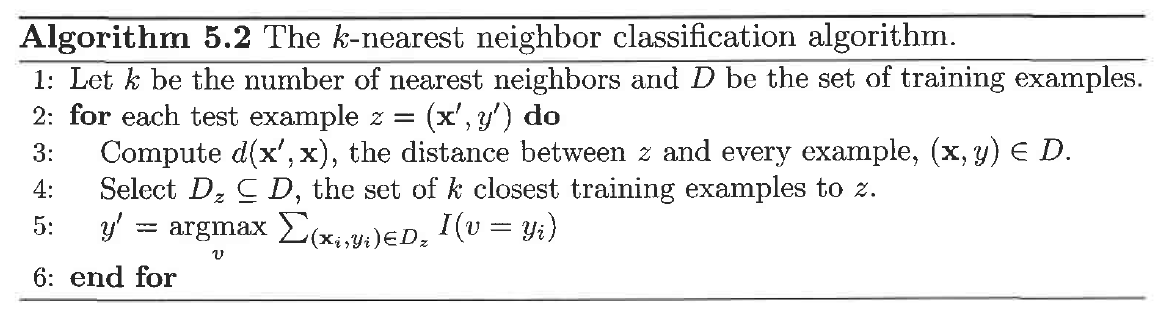
\includegraphics[width=1.0\textwidth]{images/fig1.png}
\caption{K nearest neighbors algorithm\cite{book-tan}}
\label{fig:Fig1}
\end{figure}

\subsubsection{Support in Python} 
KNeighborsClassifier is available in the scikit learn python library. 

\subsection{Logistic Regression}
Logistic regression or logit regression is a special type of regression analysis where the response variable that we need to predict is a categorical variable \cite{book-tan}. Typically logistic regression models the response variable to take two values 1 or 0, pass or fail, win or lose \cite{book-tan}. Logistic regression that takes more than two values for the response variable is called multinomial logistic regression \cite{book-tan}. Here the probability of the response variable to take a categorical value is modelled as a function of the predictor variables \cite{book-tan}. \\

Like a lot of machine learning algorithms, logistic regression works by making a lot of assumptions which should be taken care as a part of the data cleaning and transformation process \cite{book-shai}. It does not assume a linear relationship between the response variables and predictor variables \cite{book-shai}. Since it applies a log transformation on the predicted probabilities, it can handle a variety of relationship between the predictor variables \cite{book-shai}. If the predictor variables are multivariate normal, the algorithm achieves best result although it works even if they are not \cite{book-shai}. Stepwise method must be used in the logistic regression to ensure that we are neither overfitting nor underfitting the data \cite{book-shai}. A very important assumption to be noted in logistic regression is that the each attribute list must be independent, in the sense the data records must not be derived from a before-after setup experiment \cite{book-shai}. It also requires a decently large sample size to work on \cite{book-shai}. 

\subsubsection{Support for Python} LogisticRegression is available in the scikit learn python library.

\subsection{Random Forest Classifier}
Random forest is a ensemble classification algorithm which is very powerful \cite{book-tan}. Ensemble method is a special process to improve the accuracy of the prediction \cite{book-tan}. The classification algorithms we have seen so far predict the response variable using a single classifier on the test data but ensemble methods use multiple classfiers in tandem and aggregate the predictions to boost the accuracy by a huge margin \cite{book-tan}. Using a combination method, the ensemble method derives a set of base classifiers from the training data and on each iteration takes a vote of all the base classifiers to arrive at a result \cite{book-tan}. \\

Random forest is an ensemble method which works very well for classification problems \cite{book-tan}. It combines the predictions made by multiple classifiers where each classifier independently works on the training data and casts its vote \cite{book-tan}. Unlike methods like AdaBoost which generates values based on independent random vectors using a varied probability distribution, random forest generates values based on fixed probability distribution \cite{book-tan}. 

\subsubsection{Rationale for Random Forest}
Consider an example, where we have 25 base classifiers and each base classifier has an error rate of 0.35 \cite{book-tan}. As discussed, the random forest takes the majority vote given by the base classifiers \cite{book-tan}. The model makes a wrong prediction if half or more base classifiers predict wrong, if not the accuracy is improved with an error rate of 0.06 which is far better than using just a single classifier \cite{book-tan}.

\subsubsection{Support for Python} RandomForestClassifier is available in the scikit learn python library.

\section {Experiments and Results}
In this section, we will introduce the algorithm along with the details of experiments and methodology for predicting the nutrition grade of food products in France.

\subsection{Algorithm}
The problem at hand is to correctly identify the nutrition grade of the food item. The possible labels are, $a$ to $e$, with $a$ being the best and $e$ being the worst grade for a food item. For this task, we have used machine learning techniques that help in predicting the label of each food item. Before getting into the details of each step of the method, we first present a concise version of the algorithm used for this task:

\begin{enumerate}
  \item Select all the records for country, France. Drop records where nutrition grade is not populated.
  \item Separate the predictors from the response variable in order to perform data cleaning and data transformation steps.
  \item Check for missing values in the predictors obtained in the step above. Drop columns with more than 60\% missing values.
   \item Impute the missing values with 0 for remaining columns.
   \item After imputing the missing values, standardize all the numerical predictors using standard scaler.
   \item Check for the correlation between different numerical predictors. Drop one predictors from each pair of predictors that show high correlation.
   \item Combine the pre-processed predictors and the response variable in a single dataframe.
   \item Divide the data obtained in step above into training and test data using stratified sampling.
   \item Train different classifiers on the training data and check the performance of each classifier on the test data.
\end{enumerate}

\subsection{Data set}
For the classification problem, we selected the records for country France. \\ \\
Number of examples: 123,961 \\
Number of variables: 12 \\
Response variables: {\em Nutrition Grade} \\
Predictor variables: {\em Energy per 100g, Fat per 100g, Saturated Fat per 100g, Carbohydrates per 100g, Sugars per 100g, Fiber per 100g, Proteins per 100g, Salt per 100g, Trans-fat per 100g, Sodium per 100g}

\subsection{Python Packages Used}
The following Python packages were used to solve the classification problem: \\
\begin{itemize}
	\item Pandas: Provides high performance data structures for data analysis and data munging
	\item Matplotlib: Plotting library that helps embedding plots into applications using GUI 
	\item Seaborn: Visualization package based on matplotlib used for drawing high level statistical graphics 
	\item Scikit-learn: Toolbox with solid implementation of machine learning and other algorithms
	\item Scipy: Package that supports scientific computing with modules for linear algebra and integration
\end{itemize}

\subsection{Data Cleaning}
\subsubsection{Step 1: Data Sparsity} 
Data sparsity refers to the situation where a lot of attributes have missing values which is an advantage in some cases because you only need to store and analyze the data that is available to you and save on computation time and storage \cite{book-tan}. We first check the data value counts for each country. United States, France, Switzerland, Germany and Spain come as the top 5 countries with most data. Since the food nutrition grade was implemented in France, it has most products with the data available so for this classification problem we use the data filtered on France.

\subsubsection{Step 2: Handling Missing Values}
Missing values is a common scenario and they can be handled in different ways. You could choose to eliminate the data objects with missing values but at the expense of missing some critical analysis \cite{book-tan}. Estimating the missing values is also a good way to handle them, especially when the data comes from time series etc, where you could possibly interpolate the missing values from the ones that are closer to it \cite{book-tan}. Ignoring the missing values is another technique which can be applied for tasks like clustering where the similarity can be calculated using the attributes other than the missing ones \cite{book-tan}. \\

The data set was first analyzed to check the missing values in all the columns. The threshold limit has been set at 60 percent. All the columns with missing values more than 60 percent were removed from the analysis to make the result more consistent. Once the columns were removed, the data set has to be re-indexed to maintain the order. Only the columns that are important for the prediction task has been retained from the original data set. In this case, all the ingredients which are primarily the predictor variables were included. The missing values in the response variable also need to be taken care of. Removing the records with missing values for the response variable proved to be the best option after trying out various things. \\

Imputation was used to handle the null values in the predictor variables. Imputation can be done in a variety of ways with by imputing the missing values by calculating the mean and the mode or just replacing them with 0. Since all the predictor variables have numeric values, all the null values have been replaced with 0. To ensure the imputation process has been done correctly, the sum of missing values is calculated.

\subsubsection{Step 3: Outlier Treatment}
Outliers are data objects with quite distinct characteristics from the other data records \cite{book-tan}. There is a considerable difference between anomalies and outliers, where anomalies refer to data records that have bad data which is noise and need to be ignored, anomalies often contain interesting aspects and can lead to some good analysis \cite{book-tan}. In applications like {\em Fraud Detection}, anomalies could be of utmost importance \cite{book-tan}. The outliers in the data have been looked at by using box plots and have been handled as a part of the data cleaning process.

\subsection{Exploratory Data Analysis}
For exploratory data analysis, we used the Seaborn package along with Matplotlib for visualizations. The measure of spread that is the range and variance of the values is a good way to understand the different aspects of the predictor variables. Box-plots are a method of visualization to look at the distribution of values for a numerical attribute \cite{book-tan}. The box plots show the percentiles where the lower and upper ends of the box indicate $25^{th}$ and $75^{th}$ percentile, the line inside the box indicates the $50^{th}$ percentile, the tails indicate the $10^{th}$ and $90^{th}$ percentile respectively \cite{book-tan}. \\

\subsubsection{Bi-variate box-plots} Bi-variate box-plots go beyond uni-variate box plots by showing the relationship between the predictor variable and the response variable \cite{book-tan}. We look at the bi-variate box-plots for each of the important predictor variables namely saturated fat, polyunsaturated fat, sugars and salt and the response variable which is the nutrition grade. Figure \ref{fig:Fig2} shows the bi-variate box plots. \\

\begin{figure}
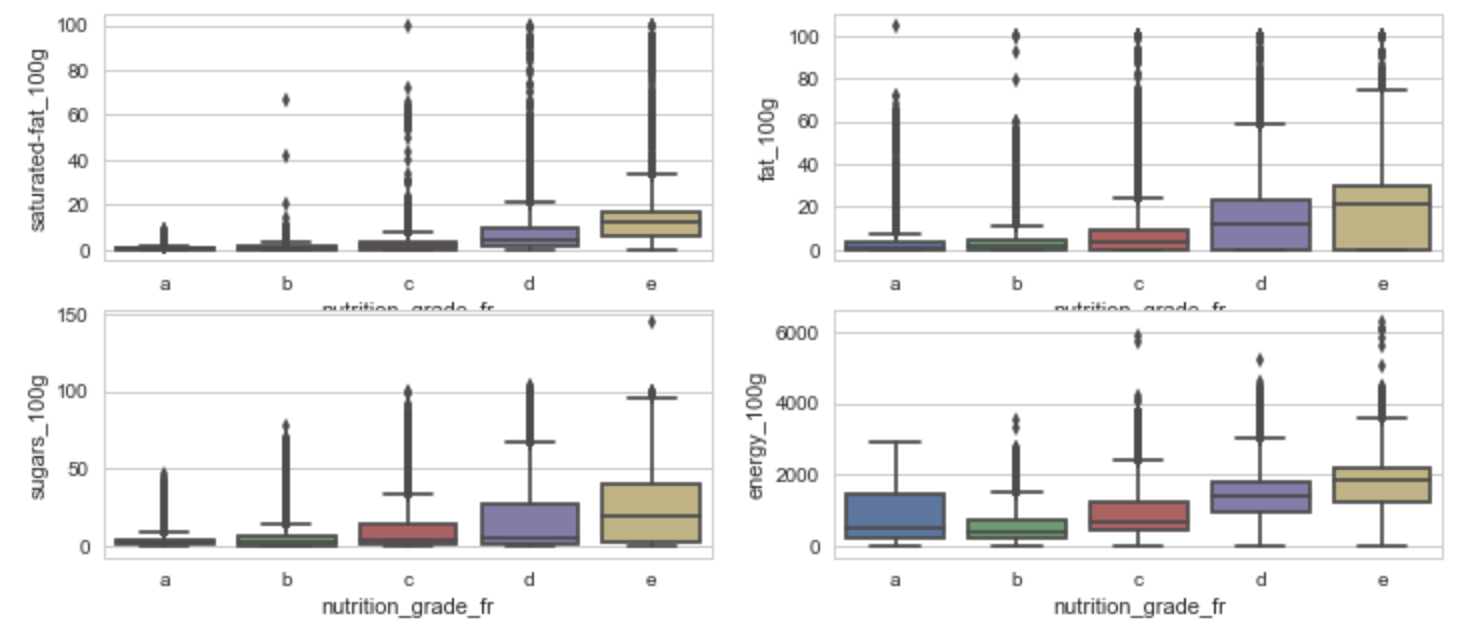
\includegraphics[width=1.0\textwidth]{images/fig2.png}
\caption{Bi-variate box plots \cite{code-base}}
\label{fig:Fig2}
\end{figure}

By looking at the box plots, we can understand some important aspects of how the response variable is related to the predictor variables. We see that as the saturated fat content increases, the food grade decreases and as the polyunsaturated fat content increases the nutrition grade is better. When the sugar levels increase the health quotient of the food comes down and the energy levels behave in a interesting manner where the energy for the nutrition grade A is higher, the energy slightly increases with the nutrition grade. While increase in energy does not necessarily imply that the nutrition quality is high because there are a lot of instant energy foods that have a lot of additives but they are often rated low when it comes to health. \\

\subsubsection{Correlation} 
Correlation between data objects is the measure of the linear relationship between the attributes of the object that are continuous variables \cite{book-tan}. Correlation analysis is the process of finding of the correlations between the different predictor variables and helps find collinearity problem \cite{book-shai}. The relationship could be either linear or non-linear given the data \cite{book-tan}. The correlation coefficient can range anywhere between -1 and 1, where 1 indicates a positive correlation and -1 indicates negative correlation \cite{book-shai}. Correlation plot visually shows the correlation coefficient between the variables in a nicely laid out plot. Figure \ref{fig:Fig3} shows the correlation plot. \\

\begin{figure}
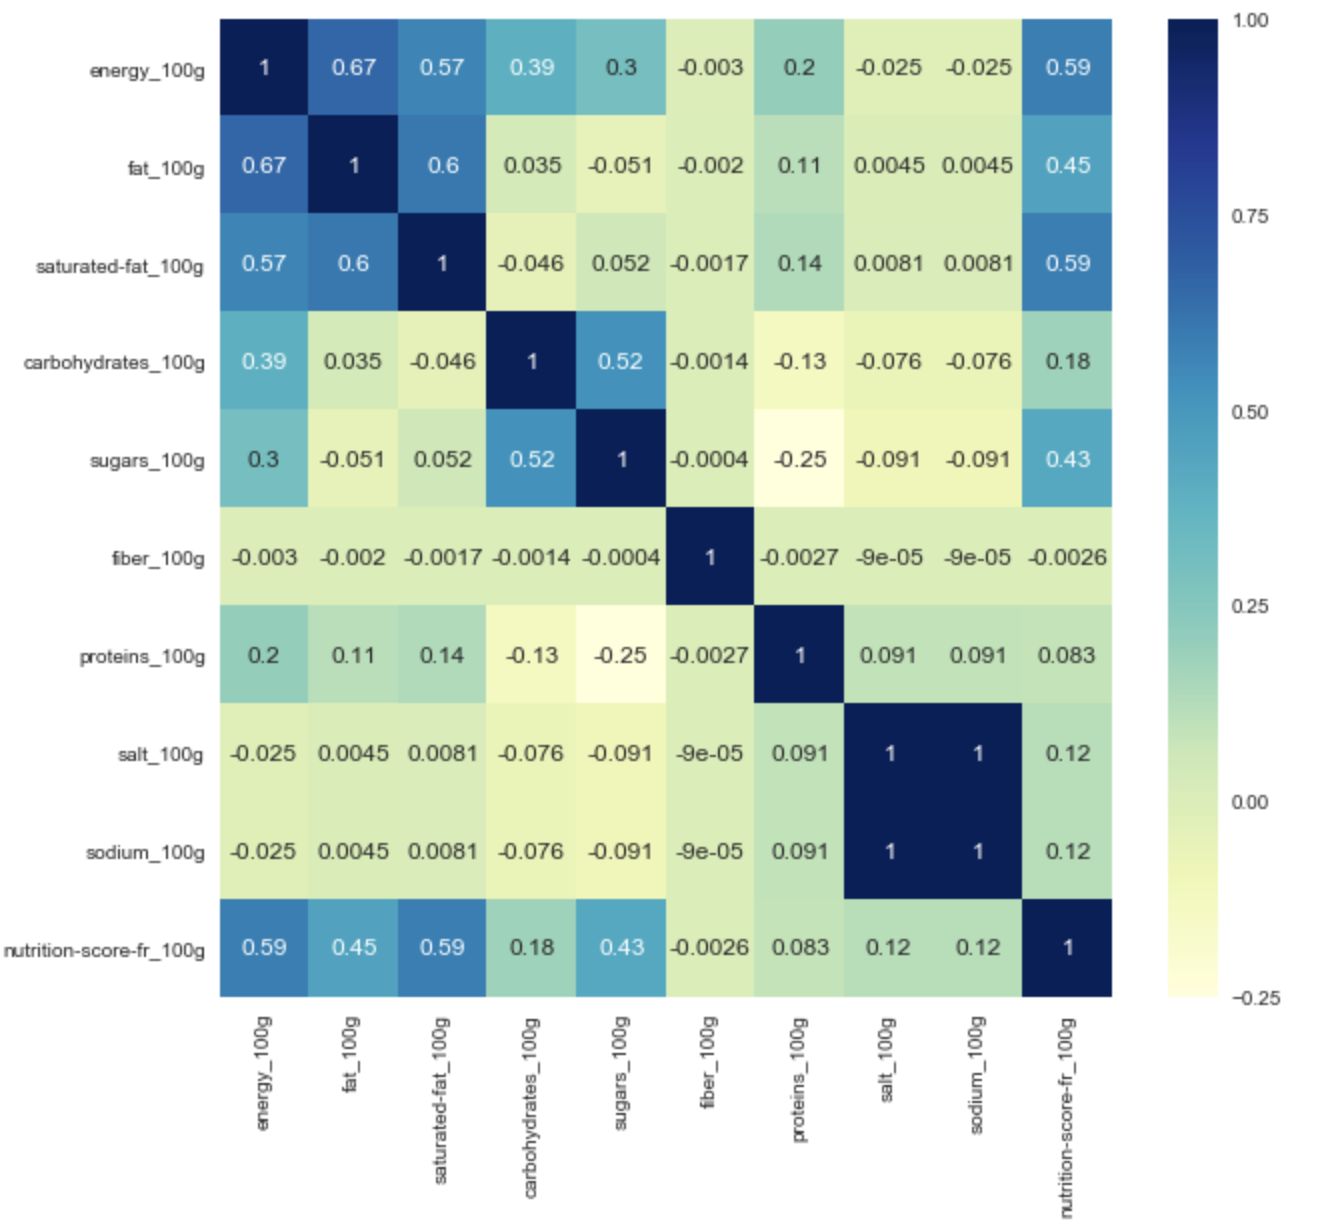
\includegraphics[width=1.0\textwidth]{images/fig3.png}
\caption{Correlation Plot \cite{code-base}}
\label{fig:Fig3}
\end{figure}

By looking at the correlation plot, we can see that sugars, fat, energy are positively in correlation with the nutrition grade. They will play an important role in the prediction algorithm. Also, sodium and salt are highly correlated with each other and this may lead to collinearity problem if not handled. Collinearity is the state where the independent variables are highly correlated with each other which can add a lot of noise to the data \cite{www-coll}. Some of the problems because of collinearity are that the regression coefficient may not be estimated correctly and also makes it very difficult to explain the response variables using the predictor variables \cite{www-coll}. So we remove sodium from the predictor variables and proceed to the next step.

\subsubsection{Data Transformation} 
Data transformation refers to the transformation that is applied to the variables \cite{book-tan}. For each data object, we apply a transformation function to all the attributes of the object to ensure that the attributes do not have a lot of variance in the data \cite{book-tan}. This process is also called standardization since we are applying a standard function to make sure all the attributes fall within a given range \cite{book-tan}. There are different methods that can be applied to achieve scaling namely log transformation, absolute value, square root transformation \cite{book-tan}. \\

We use the method called normalization where all the values fall in between the range 0 and 1. To achieve this, we use the prepossessing package from sklearn which provides utility functions and transformer classes to change raw data into a standard representation. A lot of machine learning algorithms work well on standard data. If some of the variables have extreme values, they might dominate the model function and might disturb the estimation parameter. \\

There was a massive improvement in the prediction accuracy of the algorithms before and after data scaling which proves the importance of data standardization with respect to machine learning algorithms.

\subsection{Data Sampling}
In a supervised machine learning approach, the model is trained on one sample of the data and later tested on a different sample of the data. Thus, in order to test the performance of the nutrition grade classifier, the data for the country France was divided into two samples, training and testing. There are various ways to achieve this split or sampling of the data. Some of these sampling methods are:

\begin{itemize}
	\item Simple Random Sampling: This is one of the simplest sampling techniques. In this technique, every data point has an equal chance of being selected. In other words, it works similar to a lottery system where every outcome has an equal probability. The biggest advantage of this technique is the ease of implementation and its unbiased nature while generating the sample. However, random sampling might not always result in a sample that can represent the true population. It generally works well when we have huge data to sample from.
	\item Stratified Sampling: This technique is a more sophisticated method of sampling data. Stratified sampling generates a sample such that the proportion of each class in the sample is same as that in the true population. In this technique, the entire population is divided into groups or strata. The next step is to randomly select data points from each strata such that the final sample has the same proportion for each strata as that present in the true population. Thus, the sample generated by this technique is a good representative of the true population. Stratified sampling is a very useful technique when the classes in the data are highly imbalanced. 
\end{itemize}

For our classifer, we chose to divide the data for France into training and test samples using stratified sampling technique. The strata or groups were created based on the response variable, i.e., food grade. This ensured that the training and test data had the same proportion for each food grade.

\subsection{Data Modeling}
Once the data was divided into training and test data, the next step was to train different classifiers and tune their respective parameters for better accuracy. We implemented three different models for classifying the food grade. Each of these models along with their parameters are:

\begin{itemize}
	\item K Nearest Neighbors (kNN): For kNN, the grade of a food item in test data is classified by first finding the k most similar food items in the training data. It then takes vote (food grade label) from each of these neighbors and based on the majority vote, the food item in the test data is assigned a food grade. Thus, one of the most important parameter for kNN is k, i.e., the number of neighbors to consider from the training data. We tried different k values and found that k=3 gave the best accuracy.
	\item Logistic Regression: For logistic regression, one of the important paramaters is penalty. This parameter specifies the kind of regularization to be applied. This parameter can take two possible values, $l_1$ regularization and $l_2$ regularization. Both these values penalize high magnitude of the co-efficients of the predictors in order to prevent the model from over-fitting. For our model, we have used $l_2$ regularization as it works well even in the presence of highly correlated features. 
	\item Random Forest: For random forest, there are many parameters, such as the number of trees in the forest, the maximum depth of the trees, maximum number of features to consider at each split, the minimum number of samples required in a sub-tree to qualify for further split, the minimum number of samples required to qualify as a leaf node, etc. For our data, we have kept most of the models at their default values except for the number of estimators or trees in the forest. We have set this value to 100 as the classifier produced very high accuracy with 100 trees in the forest.
\end{itemize}


\subsection{Evalution Metrics and Results}
There are various evalution metrics for assessing the performance of classifiers. Some of these evaluation metrics are \cite{hossin2015review}:
\begin{itemize}
	\item Accuracy: This metric gives the proportion of the total number of correctly classified instances
	\item Precision: This gives the proportion of the true positive instances from the total instances classified as positive
	\item Recall: This gives the proportion of the positive instances that are correctly classified
	\item F-Measure: This gives the harmonic mean between precision and the recall values
	\item Confusion Matrix: This is a useful way of checking the accuracy of the classifier. It clearly shows the number of instances correctly classified for each label. Thus, if we know that the classes in the data are not well-balanced, it's always a good idea to check the confusion matrix along with accuracy. Consider a case where 95\% of the instances belong to class A and only 5\% of the instances belong to class B. If a classifier is trained on a dataset with such imabalance, there is a high chance that the classifier would return label A for each test instance. The classifier would be still be able to correctly classify 95\% of the test instances resulting in 95\% accuracy. Thus, this is a case where accuracy can be misleading and thus a quick look at the confusion matrix can help understand the problem with the classifer. For such a case, the confusion matrix will clearly show that all the instances of the minority class, B, have been misclassified.
\end{itemize}

For our model, we used accuracy as well as confusion matrix for evaluating the results. The confusion matrix did not show any serious issues for any of the classifiers. The accuracy for each of the three classifiers was:

\begin{enumerate}
  \item Logistic Regression: With $l_2$ penalty, the accuracy of logistic regression was 78.9\%. Figure \ref{fig:Fig4} shows the confusion matrix. \\

\begin{figure}
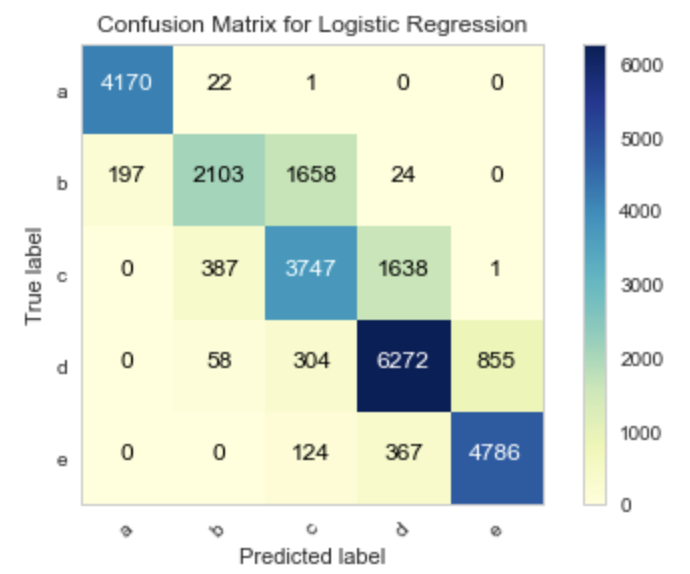
\includegraphics[width=1.0\textwidth]{images/fig4.png}
\caption{Confusion matrix for Logistic Regression \cite{code-base}}
\label{fig:Fig4}
\end{figure}

  \item K Nearest Neighbors: With k as 3, the accuracy of kNN was 95.74\%. Figure \ref{fig:Fig5} shows the confusion matrix. \\

\begin{figure}
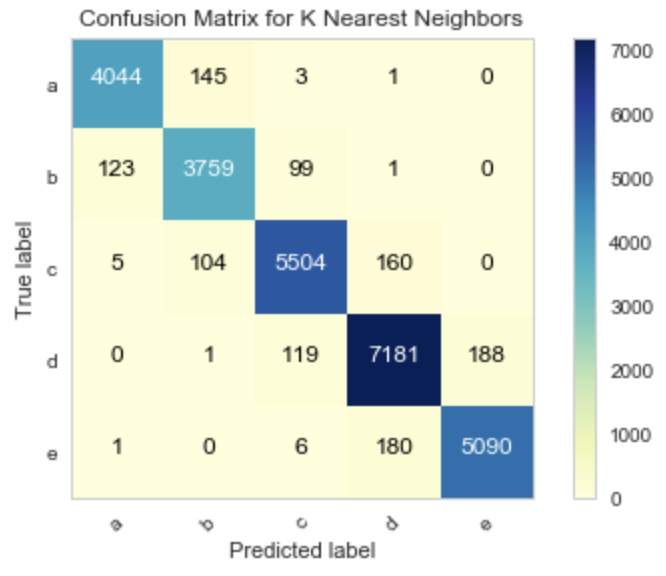
\includegraphics[width=1.0\textwidth]{images/fig5.png}
\caption{Confusion matrix for K Nearest Neighbors \cite{code-base}}
\label{fig:Fig5}
\end{figure}

  \item Random Forest: With number of trees as 100, the accuracy of random forest classifier was 99.68\%. Figure \ref{fig:Fig6} shows the confusion matrix. \\

\begin{figure}
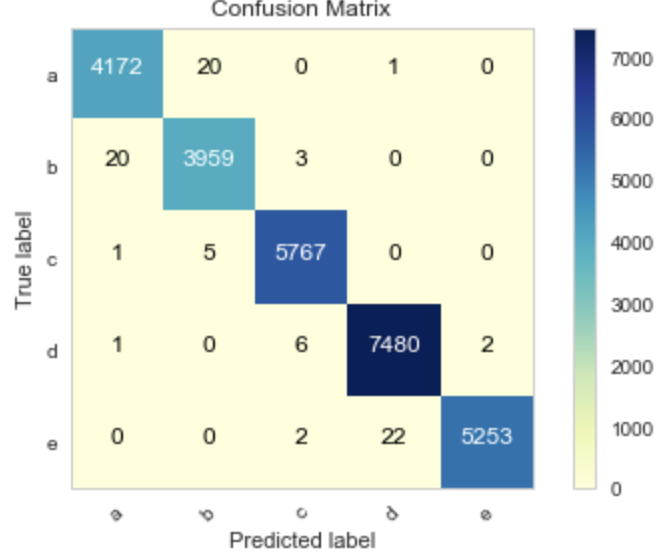
\includegraphics[width=1.0\textwidth]{images/fig6.png}
\caption{Confusion matrix for Random Forest \cite{code-base}}
\label{fig:Fig6}
\end{figure}

\end{enumerate}

Thus, we obtained the best results with Random Forest classifier.

\section{Conclusion}
Analysis of food content is very important in today's world as most of the companies try to fool consumers by labelling their product as low-fat. It's important for the consumers to know the true nutrition grade while purchasing any food item. Thus, we tried to analyze the nutrition grade based on the composition of nutritions in the food items. We tried to build a model that labels a food item purely on the basis of its nutrients without any bias such as the production company or the brand name. For accurate labeling, we applied different data cleaning and data tranformation techniques. With this transformed data, we tried various machine learning models. We got the best results using random forest classifier which was able to accurately label 99\% of the food products. Since the model is trained only for France, as part of future work, we can try and scale our model for different countries. However, to achieve similar results for other countries, we need to collect more data. The current data has many missing values for countries other than France. Once we collect enough data for these countries, we can also try and implement more sophisticated models like neural networks in future.

\begin{acks}
This project was undertaken as a part of the course objective for I523: Big Data Applications and Analytics at Indiana
University, Bloomington. We would like to thank Prof. Gregor
von Laszewski and all the TAs for their help, support and suggestions. 

\end{acks}

\bibliographystyle{ACM-Reference-Format}
\bibliography{report} 

\end{document}
